%設定頁面
\documentclass[12pt,a4paper]{article}
\usepackage[margin=1in,a4paper]{geometry}

%設定中文
\usepackage{xeCJK} 
\setCJKmainfont{標楷體} 
\XeTeXlinebreaklocale "zh"   
\XeTeXlinebreakskip = 0pt plus 1pt 

%浮水印
%\usepackage{draftwatermark}
%\SetWatermarkText{\bf NTNU MATH}
%\SetWatermarkScale{0.7}

%圖片
\usepackage{graphicx}
\usepackage{subfigure}

%頁首頁尾
\makeatother
\usepackage{fancyhdr}

%顏色
\usepackage{xcolor}

%表格顏色
\usepackage{colortbl}

%設定數學
\usepackage{amsmath, amsthm, amssymb}
\makeatletter

%自定圈圈標號
\usepackage{pstricks,pstricks-add}
\newcommand\textc[1]{{\begin{pspicture*}
(-0.25,-0.2)(0.25,0.3)\rput[c](0,0)
{\large \textcircled{\footnotesize #1}}
\end{pspicture*} }}

%自訂向量符號
\def\leftharpoonfill@{\arrowfill@\leftharpoonup\relbar\relbar}
\def\rightharpoonfill@{\arrowfill@\relbar\relbar\rightharpoonup}
\newcommand\rbjt{\mathpalette{\overarrow@\rightharpoonfill@}}
\newcommand\lbjt{\mathpalette{\overarrow@\leftharpoonfill@}}

%自訂定理
\newtheorem*{thm}{Theorem}
\newtheorem*{lem}{Lemma}
\newtheorem*{de}{Definition}
\newtheorem*{rmk}{Remark}
\newtheorem*{ex}{Example}
\newtheorem*{pf}{Proof}
\newtheorem*{sol}{Solution}

%程式碼
\usepackage{listings}
\usepackage{color}

\definecolor{dkgreen}{rgb}{0,0.6,0}
\definecolor{gray}{rgb}{0.5,0.5,0.5}
\definecolor{mauve}{rgb}{0.58,0,0.82}

\lstset{
  basicstyle={\small \ttfamily},
  frame=tb,
  language=Python,
  aboveskip=3mm,
  belowskip=3mm,
  showstringspaces=false,
  columns=flexible,
  basicstyle={\small\ttfamily},
  numbers=left,
  numbersep = 14pt,
  numberstyle=\tiny\color{gray},
  keywordstyle=\color{blue},
  commentstyle=\color{dkgreen},
  stringstyle=\color{mauve},
  breaklines=true,
  breakatwhitespace=true,
  tabsize=3,
  backgroundcolor=\color{gray!10}
}




%作者
\title{NTNU影像處理HW9}
\author{廖家緯}
\date{2020.5.13}

\begin{document}
\maketitle
%標題、作者、日期
\fontsize{12pt}{20pt}\selectfont
%設定字體大小、間距
\setlength{\baselineskip}{20pt}
%設定行距

\pagestyle{fancy}
\lhead{}
\chead{}
\rhead{}
\lfoot{}
\cfoot{\thepage}
\rfoot{}
\renewcommand{\headrulewidth}{0pt} %上線寬
\renewcommand{\footrulewidth}{0pt} %下線寬
%\renewcommand{\abstractname}{Executive Summary}




%正文開始
\begin{enumerate}
\item[•]{\bf Outline}:
\begin{enumerate}
\item[1.]Create an image $g(x,y)$ whose pixels all have the same gray value of 100. Show the image $g(x,y)$.
\item[2.]Generate Gaussian noise $n(x,y)$, with                        $\mu =0, \sigma^2 = 15$, using methods 1 and 2. Show the noisy image $f(x,y)=g(x,y)+n(x,y)$.  
\item[3.]
Display the histogram $h(i)$ of $f(x,y)$.
\item[4.]
Comment on your results.\\
\end{enumerate}

\item[•]
{\bf Code(Python):}
\begin{lstlisting}
# coding: utf-8
import numpy as np
import matplotlib.pyplot as plt
import cv2
import random
import math

n, m = 256, 256
g = (np.ones((n, m))*100).astype('uint8')

mu = 0
sigma = 15**(1/2)

#method1
f = (np.zeros((n, m))).astype('uint8')
for i in range(n):
    for j in range(m):
        if j%2 == 0:
            r, phi = random.random(), random.random()
            z1 = sigma*math.cos(2*math.pi*phi)*((-2)*math.log(r))**(1/2)
            z2 = sigma*math.sin(2*math.pi*phi)*((-2)*math.log(r))**(1/2)
            f[i, j] = g[i, j] + z1
            f[i, j+1] = g[i, j+1] + z2
            
f1 = (np.zeros((n, m))).astype('uint8')

for i in range(n):
    for j in range(m):
        if f[i, j] == 0:
            f1[i, j] == 0
        elif f[i, j] > 255:
            f1[i, j] = 255
        else:
            f1[i, j] = f[i, j]

#method2
f2 = (np.zeros((n, m))).astype('uint8')

for i in range(n):
    for j in range(m):
        s = np.random.normal(mu, sigma)
        f2[i, j] = g[i, j] + s


\end{lstlisting}

\item[•]
{\bf Input image:}\\
\begin{figure}[h]
\hspace*{1em}
\begin{tabular}{cc}

\includegraphics[height=2.5in]{image_g.jpg}&
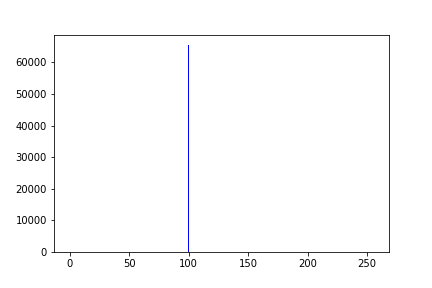
\includegraphics[height=2.5in]{g_histogram.png}\\
Input image $g(x, y)$ & Histogram of $g(x, y)$
\end{tabular}
\end{figure}

\newpage
\item[•]
{\bf Result:}
\begin{enumerate}
\item[(1)]Method 1
\begin{figure}[h]
\hspace*{1em}
\begin{tabular}{cc}

\includegraphics[height=2.5in]{image_f1.jpg}&
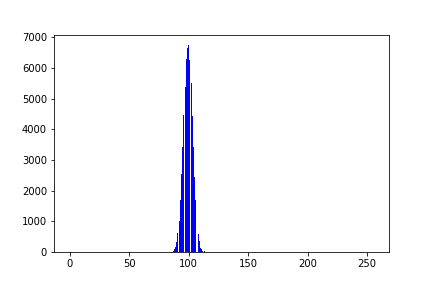
\includegraphics[height=2.5in]{f1_histogram.png}\\
Noisy image $f(x, y)$ & Histogram of $f(x, y)$
\end{tabular}
\end{figure}
 
\item[(2)]Method 2
\begin{figure}[h]
\hspace*{1em}
\begin{tabular}{cc}

\includegraphics[height=2.5in]{image_f2.jpg}&
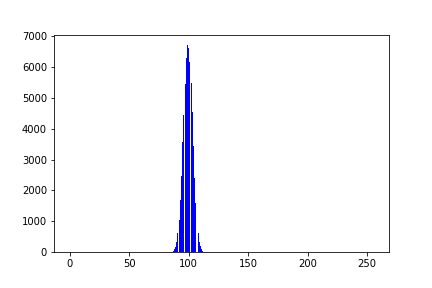
\includegraphics[height=2.5in]{f2_histogram.png}\\
Noisy image $f(x, y)$ & Histogram of $f(x, y)$
\end{tabular}
\end{figure} 
\end{enumerate}


\item[•]
{\bf Experience:}\\
這次作業花了點時間想method2的原理,我使用內建的常態分配(高斯分配)random取一個值,機率高的取到的次數多,而機率小的取到的次數小,符合老師說的機率大,對應到的區間大,機率小,對應到的區間小。從結果來看method1與method2差不多,可能$\sigma$要調整更大才會有明顯差異。
\end{enumerate}










\end{document}